%%%%%%%% ICML 2019 EXAMPLE LATEX SUBMISSION FILE %%%%%%%%%%%%%%%%%

\documentclass{article}

% use Times
\usepackage{times}
% For figures
\usepackage{graphicx} % more modern
%\usepackage{epsfig} % less modern
\usepackage{subfigure}

% For citations
\usepackage{natbib}

% For algorithms
\usepackage{algorithm}
\usepackage{algorithmic}
\usepackage{booktabs}

% As of 2011, we use the hyperref package to produce hyperlinks in the
% resulting PDF.  If this breaks your system, please commend out the
% following usepackage line and replace \usepackage{icml2019} with
% \usepackage[nohyperref]{icml2019} above.
\usepackage{hyperref}

% Packages hyperref and algorithmic misbehave sometimes.  We can fix
% this with the following command.
\newcommand{\theHalgorithm}{\arabic{algorithm}}

% Employ the following version of the ``usepackage'' statement for
% submitting the draft version of the paper for review.  This will set
% the note in the first column to ``Under review.  Do not distribute.''
% \usepackage{icml2019}

% Employ this version of the ``usepackage'' statement after the paper has
% been accepted, when creating the final version.  This will set the
% note in the first column to ``Proceedings of the...''
\usepackage[UTF8]{ctex}
\usepackage{setspace}
\setstretch{1.0}
\usepackage{lipsum}
\usepackage[accepted]{icml2019}
\usepackage{listings} % Print source code
\lstdefinestyle{python}{
    language=Python,
    basicstyle=\ttfamily\footnotesize,
    keywordstyle=\bfseries\color[rgb]{0, 0, 1},
    identifierstyle=\color[rgb]{0.5, 0.3, 0.1},
    stringstyle=\color[rgb]{0.6, 0.1, 0.1},
    commentstyle=\itshape\color[rgb]{0.05, 0.5, 0.05},
    backgroundcolor=\color[gray]{0.95},
    numbers=left,
    numbersep=5pt,
    numberstyle=\color[gray]{0.6},
    breaklines=true
}


% The \icmltitle you define below is probably too long as a header.
% Therefore, a short form for the running title is supplied here:
\icmltitlerunning{Your Awesome Project Title}

\begin{document}

\twocolumn[
\icmltitle{使用注意力机制分析多元时间序列}

% It is OKAY to include author information, even for blind
% submissions: the style file will automatically remove it for you
% unless you've provided the [accepted] option to the icml2019
% package.

% list of affiliations. the first argument should be a (short)
% identifier you will use later to specify author affiliations
% Academic affiliations should list Department, University, City, Region, Country
% Industry affiliations should list Company, City, Region, Country

% you can specify symbols, otherwise they are numbered in order
% ideally, you should not use this facility. affiliations will be numbered
% in order of appearance and this is the preferred way.
\icmlsetsymbol{equal}{*}

\begin{icmlauthorlist}
\icmlauthor{邢尚禹}{nju}
\end{icmlauthorlist}

\icmlaffiliation{nju}{Nanjing Unversity}
\icmlcorrespondingauthor{}{}

% You may provide any keywords that you
% find helpful for describing your paper; these are used to populate
% the "keywords" metadata in the PDF but will not be shown in the document
\icmlkeywords{}

\vskip 0.3in
]

% this must go after the closing bracket ] following \twocolumn[ ...

% This command actually creates the footnote in the first column
% listing the affiliations and the copyright notice.
% The command takes one argument, which is text to display at the start of the footnote.
% The \icmlEqualContribution command is standard text for equal contribution.
% Remove it (just {}) if you do not need this facility.

\printAffiliationsAndNotice{}  % leave blank if no need to mention equal contribution
% \printAffiliationsAndNotice{\icmlEqualContribution} % otherwise use the standard text.
%\footnotetext{hi}

% \begin{abstract}
% You don't need an abstract for the report.
% \end{abstract}

\section{引言}
多元时间序列指多个非独立的时间序列,对其进行预测不仅要考虑到单个变量的性质,也要正确处理变量之间的联系。论文Are Transformers Effective for Time Series Forecasting指出,Transformer在该任务上的效果不一定比最简单的单层线性网络好,这是由于时间序列的顺序非常重要,而Transformer的position embeddding对顺序并不敏感。然而,仅仅使用单层线性层并不能处理变量间的关联,对于单个变量的特征提取也仅限于线性关系。

因此,为了解决上述挑战,本文提出了使用多层线性层以及Attention机制的模型AttnLinear,能够较好地处理变量间的关联,同时也能更好地建模非线性关系。

\section{方法}
如图\ref{fg:model}所示,AttnLinear模型由线性层、Attention层、LayerNorm层、线性层组成。
\begin{figure}[htbp]
    \centering
    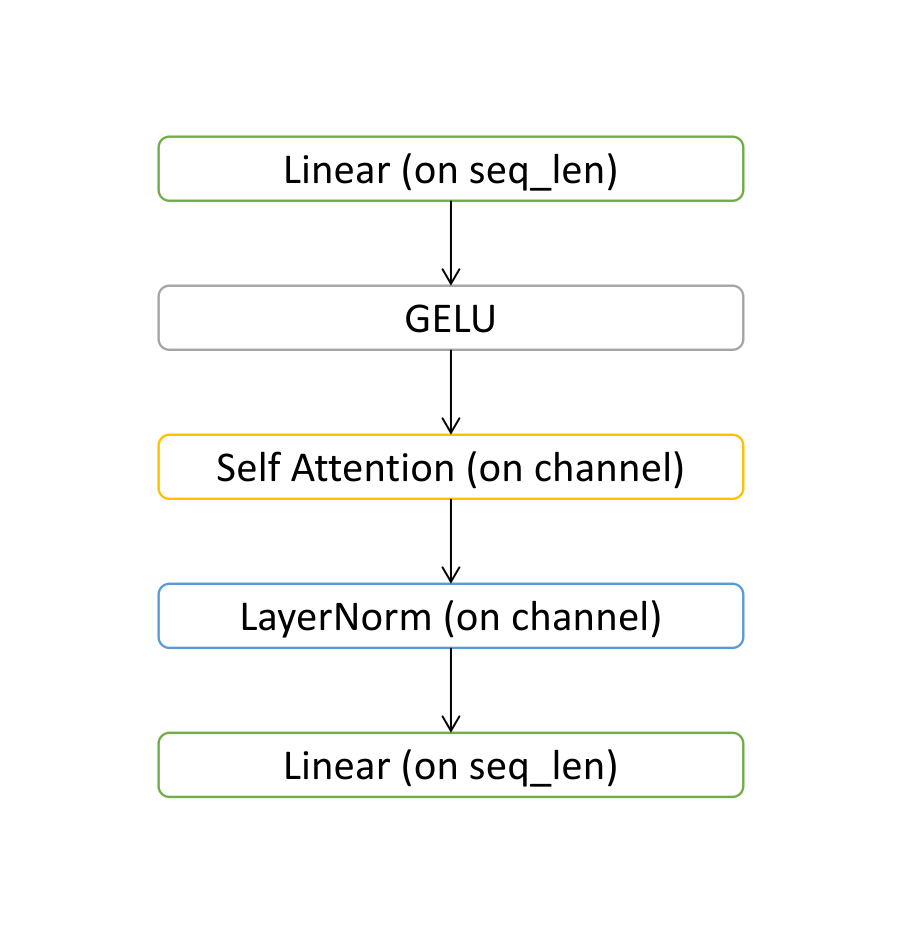
\includegraphics[width=0.45\textwidth]{model}
    \caption{模型结构}
    \label{fg:model}
\end{figure}

具体地,
\begin{enumerate}
    \item 第一层线性层,分别用weights乘以每一个channel中seq\_len长度的向量,得到长度为embedded\_size的向量,并拼接在一起;
    \item 第二层GELU是第一层线性层的激活函数;
    \item 第三层SelfAttention层,先将序列转置为[batchsize, channel, embedded\_size],再做SelfAttention,即对channel做Attention,这样可以融合不同channel的信息;
    \item 第四层LayerNorm层,对上面输出的[batchsize, channel, embedded\_size]序列做layer normlization;
    \item 第五层线性层,和第一层类似,分别用weights乘以每一个channel中embedded\_len长度的向量,得到长度为pred\_len的向量,拼接在一起输出
\end{enumerate}

这个模型能够解决上述两个挑战,这是因为
\begin{enumerate}
    \item 使用MultiHeadAttention来建模不同channel之间的关联,这样在处理一个channel时可以融合其他channel的信息;
    \item 模型是多层网络,能够建模非线性关系。
\end{enumerate}

代码实现见\ref{code}。

\begin{table}
    \label{tb:complex}
    \caption{复杂度}
    \centering
    \begin{tabular}{cccc}
        \toprule
        Method & NLinear & Transformer & AttnLinear \\
        \midrule
        Parameter  & 139.7K & 10.5M & \textbf{128.0K} \\
        Time & \textbf{10.9s} & 29.8s & 14.3s \\
        Memory & \textbf{1276MB} & 2560MB & 1456MB \\
        \bottomrule
    \end{tabular}
\end{table}

\section{实验}
为了验证该方法的性能,在三个数据集Electricity, Exchange和Weather上进行了实验。实验环境:torch1.11, python 3.10 on ubuntu22.04, NVIDIA GeForce RTX 3070 Ti Laptop GPU (8192MB)。
表\ref{tb:result}将实验结果和论文中效果最好的线性模型NLinear、效果最好的Transformer模型FEDformer进行了比较。
\begin{table*}
\label{tb:result}
\caption{实验结果}
\centering
\begin{tabular}{ccccccc}
    \toprule
    Method & \multicolumn{2}{c}{NLinear} & \multicolumn{2}{c}{FEDformer} & \multicolumn{2}{c}{AttnLinear} \\
    Metric & MSE & MAE & MSE & MAE & MSE & MAE \\
    \midrule
    Electricity-96  & \textbf{0.141} & \textbf{0.237} & 0.193 & 0.308 & 0.156 & 0.268 \\
    Electricity-192 & \textbf{0.154} & \textbf{0.248} & 0.201 & 0.315 & 0.174 & 0.285 \\
    Electricity-336 & \textbf{0.171} & \textbf{0.265} & 0.214 & 0.329 & 0.189 & 0.300 \\
    Electricity-720 & \textbf{0.210} & \textbf{0.246} & 0.355 & 0.308 & 0.218 & 0.326 \\
    Exchange-96     & \textbf{0.089} & \textbf{0.208} & 0.148 & 0.278 & 0.105 & 0.225 \\
    Exchange-192    & \textbf{0.180} & \textbf{0.300} & 0.271 & 0.380 & 0.202 & 0.327 \\
    Exchange-336    & \textbf{0.331} & \textbf{0.415} & 0.460 & 0.500 & 0.360 & 0.438 \\
    Exchange-720    & \textbf{1.033} & \textbf{0.780} & 1.195 & 0.841 & 1.078 & 0.783 \\
    Weather-96      & 0.182 & 0.232 & 0.217 & 0.296 & \textbf{0.167} & \textbf{0.228} \\
    Weather-192     & 0.225 & \textbf{0.269} & 0.276 & 0.336 & \textbf{0.212} & \textbf{0.269} \\
    Weather-336     & 0.271 & \textbf{0.301} & 0.339 & 0.380 & \textbf{0.265} & 0.316 \\
    Weather-720     & \textbf{0.338} & \textbf{0.348} & 0.403 & 0.428 & \textbf{0.338} & 0.366 \\
    \bottomrule
\end{tabular}
\end{table*}

\lstinputlisting[style=python,float=*t,label=code,title=\emph{Code 1.} 模型实现]{model.py}

表\ref{tb:result}说明,AttnLinear模型在部分数据集(例如Weather)上具有最优的表现,在其他数据集上则效果不如NLinear,但仍然优于最好的Transformer模型。这样的结果可能是由于以下几点原因:
\begin{enumerate}
    \item AttnLinear采用了多于一层的网络层,并且对于不同的channel有Attnetion交互机制,这使得其能够更好地建模非线性关系和变量间的依赖关系,导致它在部分数据集上具有最优的表现;
    \item 相比单层的NLinear, AttnLinear的多层结构可能在一定程度上影响了模型对序列顺序的关注,导致在一些数据集上效果不如NLinear;
    \item 由于时间和计算资源的限制,无法对模型进行详细的调参,只采用了和NLinear完全相同的参数,这可能也导致其无法达到最优效果。
\end{enumerate}

另外,本文也对上述几种方法的复杂度进行了评估。表\ref{tb:complex}给出了结果,其中Time代表训练一轮需要的时间,Memory代表训练过程中占用的最大显存。

\section{总结}
本文根据论文Are Transformers Effective for Time Series Forecasting,指出了目前时间序列预测模型存在的挑战,并由此设计了AttnLinear模型。AttnLinear在部分数据集上具有最优的性能,但由于没有强调对序列顺序的关注,在另外一些数据集上效果不如NLinear。
未来可以考虑添加对序列顺序的关注,设计更强大的模型。

\end{document}


% This document was modified from the file originally made available by
% Pat Langley and Andrea Danyluk for ICML-2K. This version was
% created by Lise Getoor and Tobias Scheffer, it was slightly modified
% from the 2010 version by Thorsten Joachims & Johannes Fuernkranz,
% slightly modified from the 2009 version by Kiri Wagstaff and
% Sam Roweis's 2008 version, which is slightly modified from
% Prasad Tadepalli's 2007 version which is a lightly
% changed version of the previous year's version by Andrew Moore,
% which was in turn edited from those of Kristian Kersting and
% Codrina Lauth. Alex Smola contributed to the algorithmic style files.
